\chapter{افزونه‌ها}

\section{ماشین تورینگ عصبی تکاملی}
تکامل عصبی توپولوژی‌های تقویت‌کننده\LTRfootnote{Neuroevolution of Augmenting Topologies(NEAT)} که در ادامه آن را به اختصار تکتوت می‌نامیم با یک جمعیت\LTRfootnote{Population} از شبکه‌های عصبی ساده شروع می‌کند و سپس آن‌ها را در طی نسل‌ها\LTRfootnote{Generations} با افزودن رئوس جدید و اتصالات به کمک جهش\LTRfootnote{Mutation} پیچیده‌تر می‌کند. با تکامل شبکه‌ها از این را لازم نیست توپولوژی شبکه‌ها از پیش دانسته شده باشد. تکتوت به طرز فزاینده‌ای در شبکه‌های پیچیده جستجو می‌کند تا یک سطح مناسب از پیچیدگی را پیدا کند. ویژگی مهم تکتوت این است که هم توپولوژی و هم وزن‌های یک شبکه را تکامل می‌دهد. چراکه به سادگی و تدریجی پیچیدگی را افزایش می‌دهد و این باعث می‌شود که یک شبکه مناسب با اندازه مینیمال حاصل شود.\cite{merrild2018hyperntm}
\\

بر پایه ماتع و با استفاده از تکتوت مدل ماشین تورینگ عصبی تکاملی\LTRfootnote{Evolvable Neural Turing Machine} که در ادامه آن را به طور اختصار ماتع تکاملی می‌نامیم معرفی شده است. در این روش توپولوژی و وزن‌های شبکه عصبی کنترل‌گر با کمک تکتوت یاد گرفته می‌شود. بنابراین برخلاف ماتع استاندارد نیاز به دانش پیشین\LTRfootnote{Prior Knowledge} نیست و شبکه می‌تواند باتوجه به پیچیدگی وظیفه رشد پیدا کند. ماتع تکاملی اغلب توپولوژی‌‌های فشرده برای حل یک وظیفه خاص پیدا می‌کند؛ در نتیجه جلوی جستجوی غیرضروری در فضای با ابعاد بالا گرفته می‌شود. به علاوه ماتع تکاملی قادر به جل مسائل یادگیری مستمر پیچیده است. چراکه شبکه از مشتق استفاده نمی‌کند و می‌تواند از توجه سخت\LTRfootnote{Hard Attention} و مکانیسم جابجایی\LTRfootnote{Shift Mechanism} استفاده کند که امکان تعمیم خوب برای دنباله‌های بلند در وظیفه رونوشت‌گیری را فراهم می‌کند. به علاوه یک نوار\LTRfootnote{Tape} پویا و از نظر تئوری با اندازه بی‌نهایت قابل استفاده است.\cite{merrild2018hyperntm}
\\

ماتع تکاملی یک سر تکی ترکیبی خواندن/نوشتن دارد. این شبکه بردار نوشتن $w$ با اندازه $M$، ورودی کنترل درون‌یابی\LTRfootnote{Interpolation} نوشتن $i$، ورودی کنترل پرش محتوا $j$ و سه ورودی کنترل جابجایی $s_l$ (جابجایی چپ)، $s_0$ (بدون جابجایی) و $s_r$ (جابجایی راست) را خروجی می‌دهد. اندازه بردار نوشتن $M$ اندازه هر خانه حافظه بر روی نوار را مشخص می‌کند. جزء درون‌یابی نوشتن امکان مخلوط‌کردن مقادیر فعلی نوار و بردار نوشتن در موقعیت نوشتن را فراهم می‌کند. $M_h(t)$ محتوای نوار در موقعیت سر فعلی $h$ در زمان $t$، $i_t$ درون‌یابی نوشتن و $w_t$ بردار نوشتن است. برای تمام این‌ها در زمان $t$ رابطه ۳-۱ را خواهیم داشت.\cite{merrild2018hyperntm}

\begin{equation}
M_h(t) = M_h(t − 1) · (1 − i_t) + w_t · i_t
\end{equation}

پرش محتوا مشخص می‌کند که آیا سر باید به موقعیتی در حافظه حرکت کند که بیشترین شباهت را به بردار نوشتن دارد یا نه. یک پرش محتوا انجام می‌شود اگر مقدار ورودی کنترل از ۰.۵ بیشتر شود. شباهت بین بردار نوشتن $w$ و بردار حافظه $m$‌ مطابق با رابطه ۳-۲ حساب می‌شود.\cite{merrild2018hyperntm}

\begin{equation}
s(w, m) = \frac{\sum_{i=1}^{M} |w_i−m_i| }{M} 
\end{equation}

در گام زمانی $t$ اقدامات زیر به ترتیب انجام می‌شود:
\begin{enumerate}
\item بردار نوشتن $w_t$ برای موقعیت فعلی $h$ بدست می‌آید. این بردار با محتوای موجود باتوجه به درون‌یابی نوشتن $i_t$ درون‌یابی می‌شود.
\item اگر ورودی کنترل پرش محتوا $j_t$ بزرگ‌تر از ۰.۵ شود، سر به مکانی در نوار که بیشترین شباهت به بردار نوشتن $w_t$ دارد حرکت می‌کند.
\item سر به یک موقعیت چپ‌تر، راست‌تر روی نوار حرکت می‌کند یا در همان جا ثابت می‌ماند که این وابسته به مقادیر ورودی کنترل جابجایی $s_l$، $s_0$  و $s_r$ است.
\item مقادیر نوار را در موقعیت جدید سر می‌خواند و بر می‌گرداند.\cite{merrild2018hyperntm}
\end{enumerate}

\section{ماشین تورینگ عصبی ابر تکاملی}
در کدگذاری‌های مستقیم مانند تکتوت هر بخش از نمایش جواب به یک تکه کوچک از ساختار نهایی جواب نگاشت می‌شود. عیب مهم این روش آن است که بخش‌های مختلف راه‌حل که به یک‌دیگر شبیه هستند نیز باید کد شوند و جداگانه کشف شوند. این ابراد با کدگذاری غیرمستقیم تا حد زیادی قابل حل است؛ در کدگذاری غیرمستقیم راه‌حل به شکل فشرده توصیف می‌شود و حجم اطلاعات کدشده می‌تواند کاهش بیابد. در کدگذاری غیرمستقیم به دلیل آنکه یک راه‌حل به شکل الگویی از پارامترها و نه تمام پارامترها نمایش پیدا می‌کند قدرت‌مند است.\cite{merrild2018hyperntm}
\\

روش ابر تکامل عصبی توپولوژی‌های تقویت‌کننده\LTRfootnote{Hyper Neuroevolution of Augmenting Topologies(HyperNEAT)} که در ادامه به اختصار آن را ابرتوت می‌نامیم یک افزونه از تکتوت است. در این افزونه به جای کدگذاری غیرمستقیم از کدگذاری مستقیم استفاده می‌شود. در تکتوت از شبکه‌های عصبی معمولی استفاده می‌شود درحالی که در ابرتوت از شبکه‌های تولید الگوی ترکیبی\LTRfootnote{Compositional Pattern Producing Networks (CPPN)} که در ادامه آن را به اختصار شبکه تات می‌نامیم استفاده شده است. شبکه تات برای کدگذاری ترکیب توابع طراحی شده‌اند که هر تابع در ترکیب مرتبط با یک منظم‌سازی\LTRfootnote{Regularity} است.\cite{merrild2018hyperntm}
\\

حسن شبکه تات آن است که به الگوهای مکانی اجازه می‌دهد که به عنوان شبکه‌هایی از توابع ساده نمایش پیدا کنند. این یعنی تکتوت می‌تواند با شبکه تات مانند شبکه‌های عصبی تکامل پیدا کند. شبکه‌های تات مشابه شبکه‌های عصبی هستند با این تفاوت که آن‌ها متکی بر بیشتر از یک تابع فعال‌سازی هستند.
کدگذاری غیرمستقیم شبکه تات می‌تواند به طور فشرده الگوها با نظم‌هایی نظیر تقارن\LTRfootnote{Symmetry}، تکرار\LTRfootnote{Repetition} و تکرار با تغییر\LTRfootnote{Repetition with Variation} را کد کنند. به عنوان مثال با انتخاب یک تابع گاوسین که خاصیت تقارن دارد الگوی خروجی نیز به سادگی متقارن خواهد شد. انتخاب یک تابع دوره‌ای مانند سینوس در حین تکرار قطعه‌سازی انجام می‌دهد. نهایتا تکرار با تغییر به سادگی با ترکیب یک تابع منظم (مانند سینوس یا گاوسین) با یک تابع نامنظم (مانند محور \lr{x} نامتقارن) بدست می‌آید.\cite{merrild2018hyperntm} 
\\

ایده اصلی ابرتوت آن است که شبکه‌های تات می‌تواند اتصال الگوها را کدکند. بدین طریق یک تکتوت می‌تواند یک شبکه تات که شبکه‌های عصبی بزرگ با منظم‌سازی‌ها و تقارن‌های خود نمایش می‌دهد را تکامل دهد.\cite{merrild2018hyperntm}
\\

عملکرد شبکه تات در تصویر ۳-۱ آورده شده است. شبکه‌های تات سنتی توابع هندسی هستند که الگوهای اتصال خروجی آن رئوسی در $n$ بعد است که $n$ تعداد ابعاد در فضای کارتزین است. یک شبکه تات که چهار ورودی با برچسب‌های $x_1$، $y_1$، $x_2$ و $y_2$ را دریافت کند و به عنوان خروجی مشخص می‌کند که اتصال بین نقاط دوبعدی $(x_1, y_1)$ و $(x_2, y_2)$ چه میزان است. بنابراین با داشتن یک شبکه تات آموزش یافته می‌توان با ارسال یک کوئری شامل هر دو راس در شبکه عصبی مقدار اتصال آن را بدست آورد و شبکه عصبی را ایجاد کرد.\cite{merrild2018hyperntm}

\begin{figure}[!h]
\begin{center}
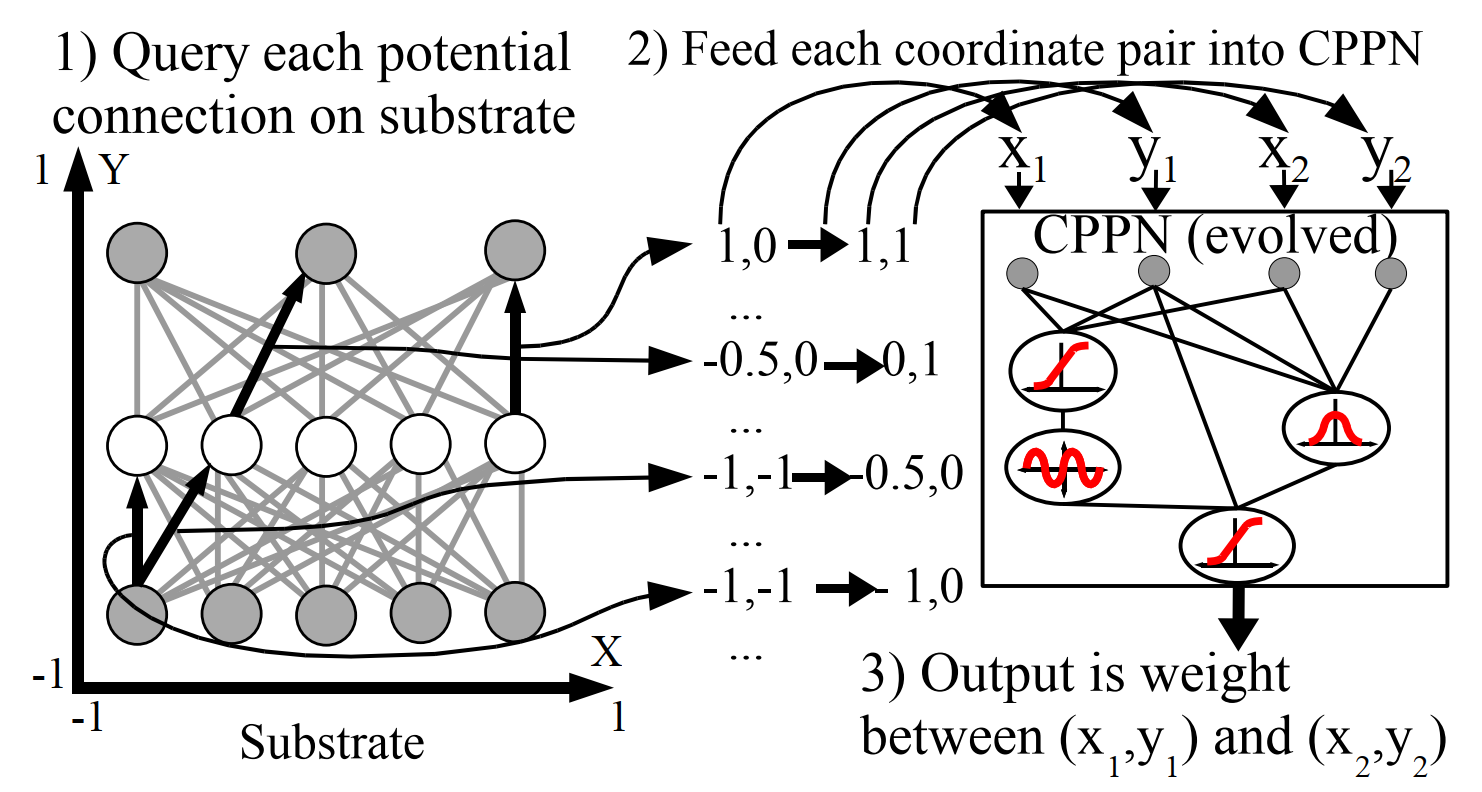
\includegraphics[height=7cm]{CPPN.png}
\end{center}
\caption{نحوه کارکرد شبکه تات\cite{merrild2018hyperntm} }
\medskip
\small
مجموعه‌ای از گره‌ها به مختصات بین -۱ تا +۱ در تمام ابعاد نظیر می‌شوند.
(۱): هر اتصال ممکن در یک شبکه عصبی کوئری زده می‌شود تا مجاورت و وزن آن مشخص شود. خطوط جهت‌دار تیره نمایش‌داده شده در تصویر یک نمونه از اتصالاتی است که کوئری زده شده است.
(۲): در درون یک شبکه تات یک گراف است که مشخص می‌کند کدام توابع فعال‌سازی به یکدیگر متصل هستند. همان‌طور که در شبکه عصبی اتصالات وزن‌دهی می‌شوند که خروجی یک تابع با چه وزنی به طرف دیگر اتصال برود، برای هر کوئری ارسال‌شده به شبکه تات جایگاه دو سر اتصال را به عنوان ورودی می‌گیرد و وزن اتصال را به عنوان خروجی می‌دهد. (۳): بنابراین شبکه تات می‌تواند الگوهای منظم از اتصالات در فضا را تولید کند.

\end{figure}

همانطور که در توضیحات قبل بدان اشاره شد باید تمام گره‌های شبکه عصبی در یک بستر\LTRfootnote{Substrate} قرار داده شوند. یعنی مشخص شود که هر گره در شبکه عصبی در چه مختصاتی در فضا باید قرار بگیرد. مشابه چیزی که در سمت چپ شکل ۳-۱ قابل مشاهده است. ایده اصلی در ماتع ابرتکاملی پیشنهاد یک بستر برای بهره‌مندی از شبکه تات در ماتع تکاملی بوده است.
\\

در مدل ماتع ابرتکاملی شبکه تات نه تنها اتصال ورودی‌ها و خروجی‌های شبکه عصبی مرتبط با وظیفه را مشخص می‌کند بلکه اینکه اطلاعات آمده از حافظه چگونه باید در شبکه ادغام شوند و چگونه اطلاعات در حافظه نوشته شوند را هم مشخص می‌کند. زیرا ابرتوت که می‌تواند هندسه یک وظیفه را یاد بگیرد قائدتا باید بتواند الگوی هندسی اطلاعات خوانده شده از و نوشته شده در حافظه را نیز یاد بگیرد.\cite{merrild2018hyperntm}
\\

شبکه ماتع تکاملی ورودی‌های زیر را دارد:
\begin{itemize}
\item \bf{شروع}: ورودی که هرگاه فعال می‌شود، ذخیره اعداد شروع می‌شود.
\item \bf{تعویض}: ورودی که هرگاه فعال شود، ذخیره اطلاعات خاتمه می‌یابد و شبکه باید مقادیر به خاطر سپرده‌شده را به یاد بیاورد.
\item \bf{ورودی بردار بیتی}: بردار بیتی که شبکه به عنوان ورودی می‌گیرد. توجه کنید قبل از آنکه ورودی تعویض فعال شود رنج این ورودی با بیت‌هایی که بعدا می‌خواند فعال می‌شود.
\item \bf{ورودی خواندن حافظه}: بردار حافظه که ماشین تورینگ در گام قبل خوانده است.\cite{merrild2018hyperntm}
\end{itemize}

این شبکه خروجی‌های زیر را هم دارد:
\begin{itemize}
\item \bf{خروجی بردار بیتی}: بردار بیتی که شبکه به عنوان خروجی می‌دهد. توجه کنید در حین دریافت ورودی این خروجی نادیده گرفته می‌شود.
\item \bf{خروجی نوشتن حافظه}: بردار حافظه‌ای که باید در حافظه نوشته شود.
\item \bf{کنترل‌گر‌های ماشین تورینگ}: خروجی‌های کنترل مخصوص ماشین تورینگ یعنی پرش، درون‌یابی و سه کنترل جابجایی (چپ، راست و توقف)\cite{merrild2018hyperntm} 
\end{itemize}

در ادامه بستر طراحی‌شده برای وظیفه رونوشت‌گیری آورده می‌شود. این بستر در شکل ۳-۲ نشان داده شده است. این بستر طراحی شده است که گره‌های ورودی بردار بیتی مختصات \lr{x} را با گره‌های نوشتن بردار حافظه به اشتراک بگذارد و بالعکس با گره‌های خواندن بردار حافظه و گره‌های خروجی بردار بیتی.
به علاوه ورودی تعویض مختصات \lr{x} اش را با خروجی پرش به اشتراک می‌گذارد بنابراین شبکه را می‌تواند وادار به پرش به حافظه‌ای کند که خواندن را از آن شروع کرده است. در این مقاله اندازه بردارهای حافظه برابر با اندازه بردار بیتی است. 
به علاوه هیچ یک از بسترها شامل گره‌های مخفی مانند آن چیزی که نشان داده شده است و ممکن است مسائل  با اندازه‌های بزرگ‌تر بدون گره مخفی را حل کند نیست.\cite{merrild2018hyperntm}


\begin{figure}[!h]
\begin{center}
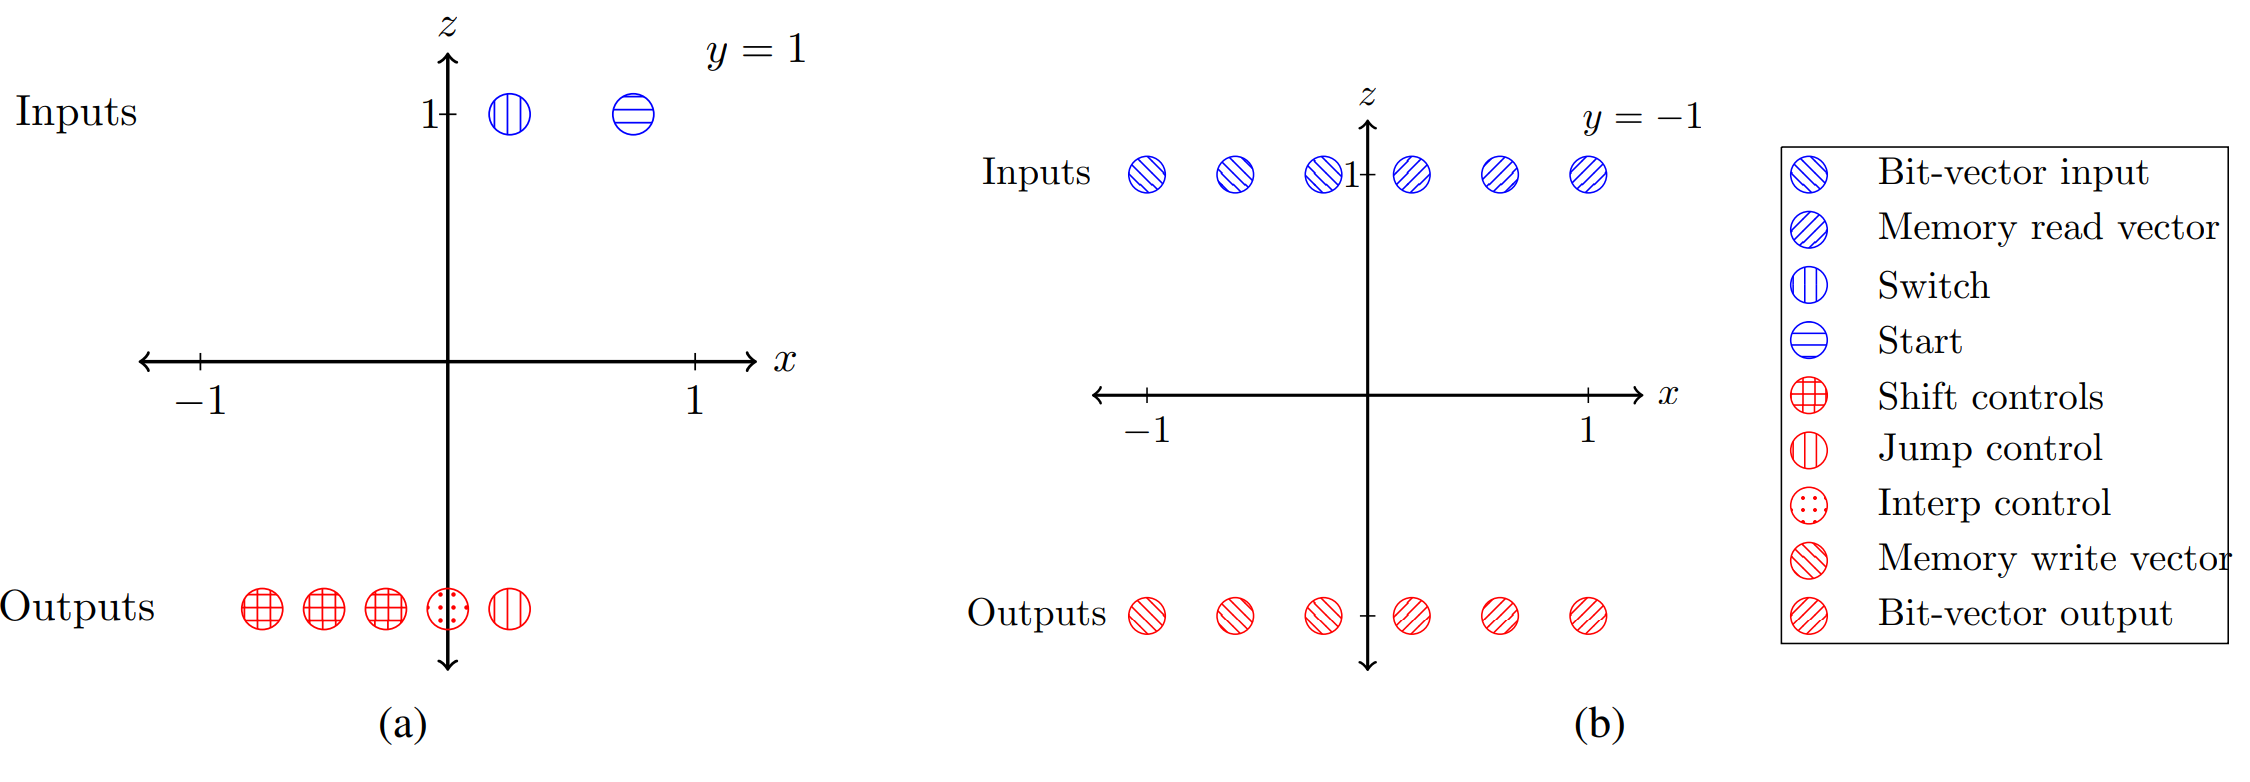
\includegraphics[height=5cm]{HyperENTM-Substrate.png}
\end{center}
\caption{بستر طراحی‌شده برای شبکه تات در مدل ماتع ابرتکاملی\cite{merrild2018hyperntm} }
\medskip
\small
تمام ورودی‌ها در $z=1$ و تمام خروجی‌ها در $z=-1$ هستند. قسمت الف تمام گره‌ها در $y=1$ را نشان می‌دهد که ورودی‌های شروع، تعویض و کنترل‌‌گرهای ماشین تورینگ هستند. لازم به ذکر است که مختصات $x$ برای ورودی تعویض و خروجی کنترل‌گر پرش یکسان است.
قسمت ب گره‌ها را در $y=-1‌$ نشان می‌دهد که ورودی و خروجی‌های بردار حافظه و بردار بیتی را نشان می‌دهد. گره‌های ورودی بردار بیتی مختصات $x$ را با گره‌های نوشتن بردار حافظه به اشتراک می‌گذارد، درحالی‌که گره‌های خواندن بردار حافظه مختصات $x$ را با گره‌های خروجی بردار بیتی به اشتراک می‌گذارد.\cite{merrild2018hyperntm}
\end{figure}

در کنار خروجی شبکه تات که وزن هر اتصال را مشخص می‌کند، هر شبکه تات یک خروجی تابع قدم\LTRfootnote{Step Function} اضافه دارد که خروجی بیان پیوند نامیده می‌شود. این خروجی مشخص می‌کند که آیا یک اتصال باید بیان شود یا خیر. اتصالات بالقوه برای هر ورودی در لایه‌های $y=1$ و $y=-1$ به هر خروجی در لایه‌های $y=1$ و $y=-1‌$ کوئری زده می‌شود. تعداد ورودی‌ها و خروجی‌ها در لایه $y=-1$ مطابق قسمت ب تصویر ۳-۲ وابسته به اندازه بردار بینی وظیفه رونوشت‌گیری است، که در مثال نشان‌داده شده اندازه بردار بیتی برابر با ۳ است. نورون‌ها به شکل یکنواخت در بازه‌های -۱ تا -۰.۲ در مختصات $x$ برای ورودی‌های بردار بیتی و بردار نوشتن حافظه استفاده می‌شود و بازه ۰.۲ تا ۱ برای بردار نوشتن حافظه و خروجی بردار بیتی استفاده می‌شود.\cite{merrild2018hyperntm} 
\\

نهایتا برای تعیین میزان بایاس یک گره باید مختصات همان گره را هم به عنوان گره مبدا و هم به عنوان گره مقصد به شبکه تات کوئری زد.\cite{merrild2018hyperntm}

\section{ماشین تورینگ عصبی متوجه}
در مدل ماتع متوجه حافظه با یک مکانیسم آدرس‌دهی وابسته به محتوا بازیابی می‌شود. آدرس‌دهی برپایه محتوا به صورت ضروری یک گام محاسبه شباهت میان بردار خروجی کنترل‌گر $C_t$ و بردارهای حافظه موجود $M_t$ است. وزن توجه در خواندن با رابطه ۳-۳ تولید می‌شود. در رابطه مذکور متغیر $\beta$ می‌تواند دقت تمرکز را افزایش یا کاهش دهد و معیار شباهت استفاده‌شده معیار شباهت کسینوسی است.\cite{zhao2020cold}

\begin{equation}
w_t^r(i) = \frac{exp(\beta.sim(C_t,M_t(i)))}{\sum_j(exp(\beta.sim(C_t,M_t(j))))}
\end{equation}

در حالت کلی کنترل‌گر می‌تواند با هر شبکه عصبی مصنوعی طراحی شود. در ماتع متوجه از یک لایه توجه چندسر\LTRfootnote{Multi-Headed Attention} استفاده کرده‌اند تا روابط بین دنباله‌های ورودی و خروجی را مدل کنند. \cite{zhao2020cold}
\\

رابطه مربوط به لایه توجه در رابطه ۳-۴ آورده شده است. در این رابطه مطابق معمول $K$، $Q$ و $V$ به ترتیب ماتریس کوئری، کلید و مقدار است و $n$ تعداد ابعاد است. توجه بر دنباله ورودی $I$ اعمال می‌شود تا یک جمع وزن‌دار برای هر $i_t$ بر پایه $i_1$ تا $i_t$ اعمال شود که $t$ زمان فعلی است.\cite{zhao2020cold} 

\begin{equation}
Attention(Q,K,V) = softmax(\frac{QK^T}{\sqrt{n}})
\end{equation}

به عنوان خروجی مدل یک بردار وزن مرتبط با هر تلاش را یاد می‌گیرد و بردار وزن یادگرفته‌شده برای محاسبه پیش‌بینی خروجی $i_t$ استفاده می‌شود. از تابع خطا میانگین مربعات خطا مطابق رابطه ۳-۵ استفاده می‌شود. در این رابطه $a_t^k$ مقدار پیش‌بینی، $gt_t^k$ مقدار واقعی برچسب، $b$ اندازه دسته\LTRfootnote{Batch}، $k$ طول دنباله و $t$ زمان است.\cite{zhao2020cold}

\begin{equation}
L = \sum_b \sum_{k=1}^n \sum_{t=1}^T MSE(a_t^k, gt_t^k)
\end{equation}

در ماتع متوجه حافظه با مکانیسم آدرس‌دهی برپایه موقعیت بروز می‌شود. مکانیسم آدرس‌دهی برپایه موقعیت برای چندین گام طراحی شده است تا تکرار بر روی خانه‌های حافظه و پرش‌های دسترسی تصادفی را امکان‌پذیر کند. گام اول محاسبه درون‌یابی بین بردار وزن نوشتن پیشین $w_{t-1}$ و بردار وزن محتوا تولیدشده توسط مکانیسم آدرس‌دهی محتوا $w_t^c$ در گام زمانی فعلی با استفاده از دروازه\LTRfootnote{Gate} درون‌یابی $w_t^g$ مطابق رابطه ۳-۶ است.\cite{zhao2020cold}

\begin{equation}
w^g_t = g_t ∗ w^c_t + (1−g_t) ∗ w_{t−1}
\end{equation}

بعد از درون‌یابی یک وزن‌دهی جابجایی $s_t$ بر ماتریس وزن دروازه‌دار با یک کانولوشن دایره‌ای برای تنظیم حافظه مطابق رابطه ۳-۷ اعمال می‌شود. در این رابطه $N$ برابر با اندازه حافظه است. نهایتا مطابق رابطه ۳-۸ عمل تیزکردن\LTRfootnote{Sharpen} برای نرمال‌سازی استفاده می‌شود.\cite{zhao2020cold}

\begin{equation}
w_t^{ro} = \sum_{j=0}^{N-1}w_t^g(j)s_t(i-j)
\end{equation}

\begin{equation}
w_t(i) = \frac{w_t^{ro}(i)}{\sum_j w_t^{ro}(j)}
\end{equation}

\section{ماشین تورینگ عصبی پویا}
